
\section{방법론}
\subsection{프레임워크 설계}

% The proposed framework, illustrated in Figure~\ref{fig:engine}, facilitates multi-agent coordination through interconnected modules that \textbf{support adaptive collaboration}, effective communication, and strategic task execution. Central to this framework is the \textbf{Coordination Engine}, which orchestrates the following primary modules: \textbf{Agent Graph}, and \textbf{Cognitive Module}, more details about different modules can be found on Appendix \ref{framework}. \kunlun{specifying more modules shown on Appendix A.1, citing the graphics}


% \paragraph{Agent Graph Module}
% Transforms configuration data into a graph $G = (V, E)$, where each node $v_i \in V$ represents agent $A_i$, and edges $e_{ij} \in E$ denote relationships like collaboration $(A_i \leftrightarrow A_j)$, supervision $(A_i \rightarrow A_j)$, or negotiation $(A_i \leftrightsquigarrow A_j)$. This graph informs the coordination protocol and underpins collective reasoning and decision-making.

% \kunlun{specify the need and the design of Agent graph}



% \paragraph{Cognitive Module and Communication Module }
% \kunlun{social, relationship aware and memory design}
% Handles internal reasoning and strategic decision-making by integrating shared and individual memories, environment observations, and agent relationships from the graph. Inspired by theory-of-mind, it allows agents to infer others’ intentions and roles, promoting socially intelligent behavior. This module manages prompt construction for reasoning, reflection, and summarization, refining understanding of social structures and communication patterns to adapt strategies over time.
% \kunlun{strength how these modules enable the coordination and competition}

% Two agents $A_i, A_j$ can communicate with each other if $(v_i, v_j) \in G$. Agents are presented the option of communicating with another agent with the communication option provided as a tool. They are also given profiles of the agents they can communicate to, so they can choose which agent to talk to. Then two agents will have a conversation between them until they decide to terminate or the communication exceeds allowed rounds. Finally, the conversation will be summarized and inserted into the Memory of the two agents.
% \paragraph{Coordination Engine & Action Modeule}
% \kunlun{adding function calling style of tool calling citing tool work for actions}
% Guides the execution flow by initializing agents, tasks, and relationships via the Configuration Module, constructing the agent graph with the Agent Graph Module, and preparing the environment and its tool functionalities. Agents then interact with the environment through cognitive processing and memory retrieval, with observations and results updating both memory and cognitive states. The engine iteratively refines agent states and strategies, ensuring continuous learning and enhancement of coordination and task execution efficacy. Upon reaching task-specific milestones or termination conditions, the final results are returned to the evaluator, which provides performance feedback and updates key performance indicators.

% \kunlun{also writing the paragraph how the agents running and coordination within our framework from the relationship to the results how we save then evaluate them. Predefined agents and flixible executing structures: how the whole thing executed}

우리가 제안하는 평가 프레임워크 MARBLE~(Figure~\ref{fig:engine} 참조)은 adaptive collaboration, efficient communication, strategic task execution을 가능하게 하는 상호연결 모듈을 활용하여 강건한 다중 에이전트 조정 시스템을 구축한다. 그 핵심에는 시스템 전반의 매끄러운 상호작용을 보장하기 위해 \textit{Agent Graph}, \textit{Cognitive Module}, \textit{Coordinate Engine}을 포함한 주요 모듈을 초기화하고 동기화하는 \textit{Coordination Engine}이 있다. 추가 모듈의 자세한 설명은 Appendix~\ref{framework}에서 확인할 수 있다.

% \paragraph{Agent Graph Module}
% This module transforms configuration data into a structured graph $G = (V, E)$, where each node $v_i \in V$ represents an agent $a_i$, and each edge $e_{ij} \in E$ encodes various inter-agent relationships such as collaboration $(a_i \leftrightarrow a_j)$, supervision $(a_i \rightarrow a_j)$, or negotiation $(a_i \leftrightsquigarrow a_j)$. \kunlun{refine the math annotation}The design of the Agent Graph is pivotal for capturing dynamic interaction patterns and ensuring scalable coordination across agents. \kunlun{using the agent1 rel agent2 to form the graph, when communicate only communicate with someone with relationship which like in the real-world}

\paragraph{Agent Graph Module}
이 모듈은 configuration data를 구조화된 그래프 \(G = (\mathcal{A}, E)\)로 변환한다. 여기서 \(\mathcal{A} = \{a_1, a_2, \dots, a_n\}\)는 에이전트 집합을 나타내며, \(E\)의 각 edge는 \(r \in \mathcal{R}\)이 에이전트 \(a_i\)와 \(a_j\) 사이의 관계를 나타내는 triple \((a_i, r, a_j)\)로 정의된다. 예를 들어 협업 관계는 \((a_i, \texttt{collaborates}, a_j)\), 감독은 \((a_i, \texttt{supervises}, a_j)\), 협상은 \((a_i, \texttt{negotiates}, a_j)\)로 표기한다. 이러한 triple 관계를 기반으로 그래프를 구성함으로써, 이후의 의사소통과 조정이 명시적으로 정의된 관계를 가진 에이전트 사이에서만 일어나도록 하며, 이는 실제 세계의 상호작용 패턴을 반영한다.


% \paragraph{Cognitive Module}
% The Cognitive Module underpins internal reasoning by integrating shared and individual memories, real-time environmental observations, and relational data from the Agent Graph. Inspired by cognitive theories of self-reflection and theory-of-mind \citep[e.g.,][]{premack1978}, this module generates expected outcomes and progress for each task and stores them in memory. In subsequent iterations, actual performance is compared against these expectations to produce evolving experiences. These experiences guide adjustments in planning, enabling agents to continuously refine their strategies and adapt to unexpected outcomes. \kunlun{cognitive module in responsible agent evolving, and social intelligence important for the multiagent coordination, with agent self involving persona, agent relationship, its intter action reasoning method(cot, react, ..) updating its memory, social aware etc}

\paragraph{Cognitive Module}
Cognitive Module은 다중 에이전트 조정에서 책임 있는 에이전트 진화와 사회적 지능의 중심이다. 이 모듈은 각 에이전트의 persona, 에이전트 간 관계, Chain-of-Thought~\citep{wei2023chainofthoughtpromptingelicitsreasoning} 및 ReACT~\citep{yao2023reactsynergizingreasoningacting} 같은 추론 전략을 포함하는 포괄적 내부 상태를 유지하고 갱신한다. 핵심적으로 이 접근은 인간이 사회적 단서, 과거 경험, 맥락 정보를 바탕으로 정신 모델을 지속적으로 갱신하는 방식과 유사하게, theory-of-mind와 social intelligence의 요소를 결합하여 인간의 인지 과정을 모사한다 \citep[e.g.,][]{premack1978}. 인지적, 사회적, 적응적 메커니즘의 결합은 우리 시스템의 중추를 형성하며, 에이전트가 복잡한 환경에서 전략을 동적으로 조정하고 협업적으로 진화할 수 있게 한다.


\begin{figure*}[ht]
    \centering
    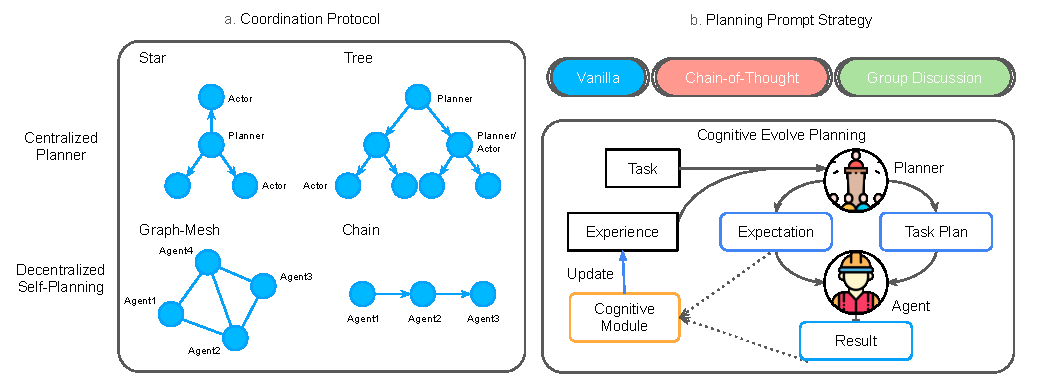
\includegraphics[width=\textwidth]{graphs/coordination.pdf}
    \caption{\textbf{조정 프로토콜과 planning prompt 전략의 예시}.
    \textbf{(a)}는 star, tree, graph, chain 같은 centralized 및 decentralized planning 구조를 보여 준다.
    \textbf{(b)}는 효과적 planning을 위해 iterative feedback과 task update를 통합하는 group discussion 및 cognitive prompt 같은 전략을 설명한다.}
    \label{fig:coordination}
\end{figure*}

% \subsubsection{Coordination Engine}
% The Coordination Engine orchestrates the overall execution flow of the system. It initializes agents, tasks, and inter-agent relationships via a dedicated Configuration Module and constructs the Agent Graph to represent these dynamics.

% \kunlun{define what is a planner within the coordination engine and what is an actor, a planner plans the task input for the actor, actor is the agent within the Agent Graph and can use tools interact with the env or other agents}

% \kunlun{define 4 coordination protocol clear below}


%  Our approach considers four Coordination protocol---\textbf{star}, \textbf{tree}, \textbf{graph}, and \textbf{chain}. Specifically, \textbf{star} and \textbf{tree} are centralized methods where one (or a hierarchy of) planner(s) manages task allocation and aggregates feedback, while \textbf{graph} and \textbf{chain} rely on decentralized coordination through peer-to-peer interactions and sequential task handoffs.

% \paragraph{Centralized Coordination: Star \& Tree.}
% In the \textbf{star} configuration, a single central planner assigns tasks to all agents and consolidates their feedback, making it effective for tasks that require strong oversight but potentially limited in scalability. The \textbf{tree} structure builds on this by organizing agents hierarchically: a top-level planner delegates tasks to subordinate planners, combining centralized control with enhanced scalability for complex tasks.

% \paragraph{Decentralized Coordination: Graph \& Chain.}
% The \textbf{graph} configuration utilizes a network of interconnected agents that communicate directly, enabling concurrent planning and distributed decision-making. In contrast, the \textbf{chain} structure arranges agents sequentially, where each agent passes decisions to the next. This approach is well-suited for tasks with sequential dependencies, though it may constrain parallel processing.

% \paragraph{Planner Design and Enhancements.}
% \kunlun{updating the new method of cognitive evolving with expectation result and experience update for better task  planning }
% \kunlun{for the star coordination style, ablation on different planning stratigies}
% Building on these structures, our approach employs iterative, feedback-driven planning. A zero-shot chain-of-thought prompt equips the planner with the target task, agent profiles, \heng{not sure what agent profile contains, define and give example} and a summary of past subtasks, enabling step-by-step reasoning. The REACT-style mechanism interleaves planning with action, while \textbf{group discussions} allow agents to share insights and constraints. \textbf{Cognitive planning} principles further ensure effective workload distribution and task alignment. Each round concludes with a concise summary of lessons learned, continuously refining the system's coordination and performance.  \kunlun{For cognitive evolve, when generating a task, the expected result and progress are produced and stored in memory; in subsequent iterations, the actual progress is compared with the expectations to generate evolving experiences that inform adjustments to planning if the outcomes fall short, with these experiences continually saved and updated to guide future plans.}

\subsubsection{Coordination Engine}
Coordination Engine은 시스템의 전체 실행 흐름을 조율한다. 전용 Configuration Module을 통해 에이전트, 과제, 에이전트 간 관계를 초기화하고, 이러한 동역학을 표현하기 위해 Agent Graph를 구성한다. 우리의 프레임워크에서는 두 가지 핵심 역할인 \emph{planners}와 \emph{actors}를 구분한다. Planners는 과제 입력을 설계하고 전략을 수립하며 전체 과제 할당을 관리하고, Agent Graph 안에 표현되는 actors는 사용 가능한 도구를 통해 환경 및 다른 에이전트와 상호작용하면서 과제를 실행한다.

우리 접근은~\citet{qian2025scaling}의 연구와 유사하게 \textbf{star}, \textbf{tree}, \textbf{graph}, \textbf{chain}이라는 네 가지 구별되는 coordination protocol을 지원한다.

% The \textbf{star} and \textbf{tree} configurations adopt centralized coordination, where one (or a hierarchy of) planner(s) manages task allocation and aggregates feedback from actors. In contrast, the \textbf{graph} and \textbf{chain} configurations rely on decentralized coordination through peer-to-peer interactions and sequential task handoffs.

\paragraph{Centralized Coordination: Star \& Tree.}
\textbf{star} 구성에서는 단일 중앙 planner가 모든 actor에게 과제를 할당하고 그들의 feedback을 통합하여 강한 감독을 제공하지만, scalability를 제한할 수 있다. \textbf{tree} 구조는 에이전트를 계층적으로 조직하여 이를 확장한다. 최상위 planner가 하위 planner에게 과제를 위임하고, 하위 planner는 다시 actor와 조정한다. 이러한 계층적 접근은 더 복잡한 과제를 처리하기 위해 centralized control과 향상된 scalability 사이의 균형을 맞춘다.

\paragraph{Decentralized Coordination: Graph-Mesh \& Chain.}
\textbf{graph-mesh} 구성은 서로 연결된 actor들의 네트워크를 사용하며, actor들이 직접 의사소통하도록 하여 concurrent planning과 distributed decision-making을 가능하게 한다. 반대로 \textbf{chain} 구성은 actor를 순차적으로 배열하고 각 에이전트가 자신의 결정을 다음 에이전트에게 전달하게 한다. 이러한 순차 handoff는 내재적 의존성이 있는 과제에 적합하지만 병렬 처리 능력을 제한할 수 있다.

% \paragraph{Planner Design and Enhancements.}
% In centralized coordination, building on these coordination protocols, our system employs iterative, feedback-driven planning. The planner leverages a zero-shot chain-of-thought prompt that includes the target task, detailed agent profiles (such as roles, expertise, and historical performance), and summaries of previous subtasks to facilitate step-by-step reasoning. A REACT-style mechanism interleaves planning with execution, while group discussions enable agents to share insights and constraints. Moreover, our cognitive planning method generates expected outcomes and progress for each task and stores these in memory. In subsequent iterations, actual performance is compared against these expectations to produce evolving experiences that guide adjustments in planning. \kunlun{see appendix for detailed prompting.} This continuous process of self-reflection and adaptation enhances coordination efficiency and has been validated through ablation studies on the star coordination style.

\paragraph{Planner Design and Enhancements.}
우리의 centralized coordination protocol에서 planner는 인간의 의사결정 과정을 반영하는 네 가지 planning 접근, 즉 vanilla prompting, chain-of-thought (CoT)~\citep{wei2022chain}, group discussion, cognitive self-evolving planning을 지원한다. \textbf{vanilla prompt}는 직관적인 zero-shot 지시를 사용해 task plan을 직접 생성한다. \textbf{CoT approach}는 target task, roles, expertise, historical performance를 포함한 agent profiles, 이전 subtask 요약 같은 상세 입력을 통해 단계별 추론을 촉진하여 논리적 진행을 이끈다. \textbf{group discussion}~\citep{chen2023agentversefacilitatingmultiagentcollaboration} 방법은 여러 에이전트가 통찰과 제약을 공유하도록 하여 전체 계획을 다듬는 협업적 숙의를 촉진한다. 마지막으로 Reflexion~\citep{shinn2023reflexion} 방법과 유사하게, 우리의 \textbf{cognitive self-evolving planning} 방법은 각 과제의 기대 결과와 진행을 생성해 memory에 저장하고, 이후 반복에서 실제 성능을 이러한 기대와 비교함으로써 인간의 학습을 모사한다. 이 비교는 evolving experience를 만들어 미래 planning을 지속적으로 알리고 조정한다(자세한 prompting은 Appendix~\ref{sec:important-prompts} 참조). 이 방법들은 함께 개별 추론과 협업적 최적화를 모두 활용하며, star coordination style에 대한 ablation study에서 검증된 것처럼 조정 효율을 높인다.





\subsection{벤치마크 설계}

\begin{figure*}[ht]
    \centering
    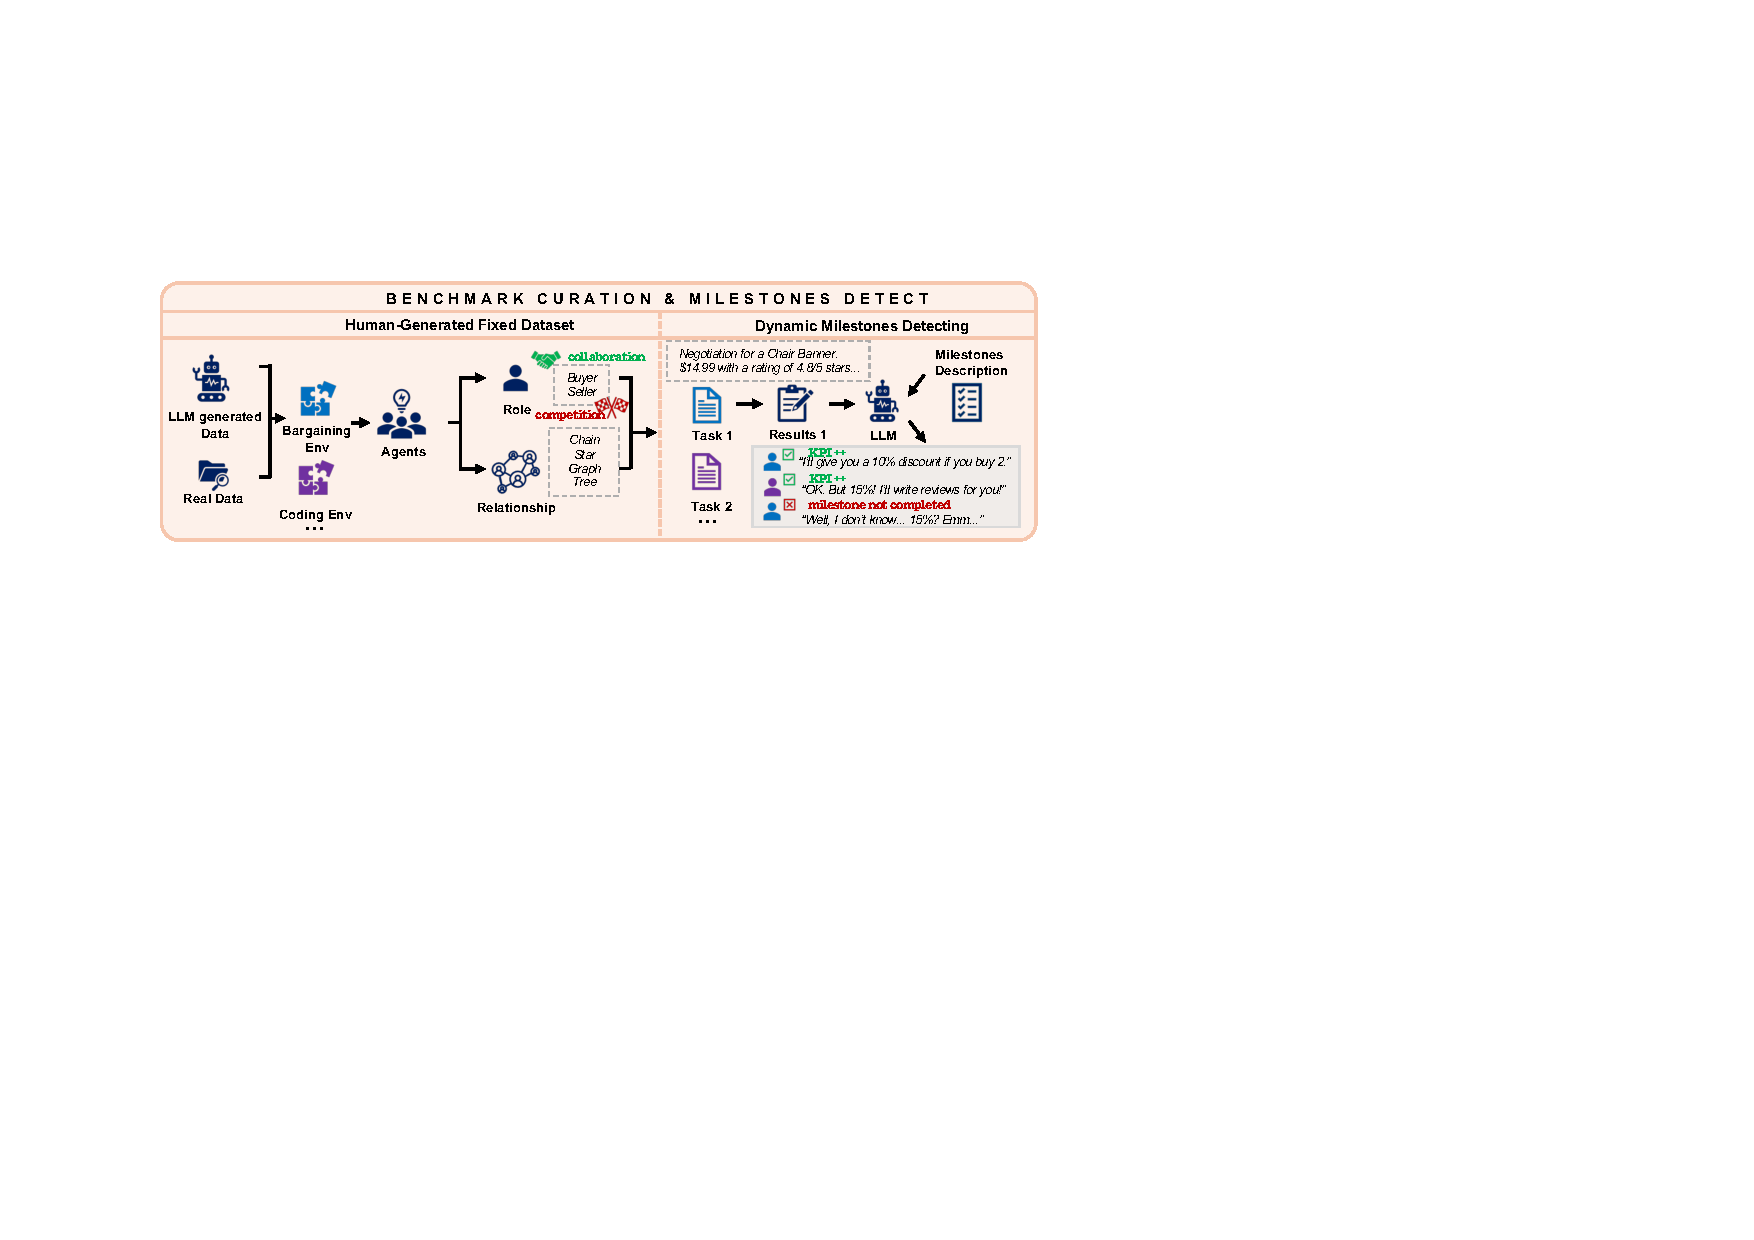
\includegraphics[width=\textwidth]{graphs/marble_graph.pdf}
    \caption{우리의 benchmark curation과 KPI metric을 위한 dynamic milestone detection의 예시.}
    \label{fig:method}
\end{figure*}

우리의 다중 에이전트 프레임워크를 체계적으로 평가하기 위해, \textit{task-oriented} 및 \textit{social-simulation-based} 환경을 포괄하는 다양한 시나리오의 벤치마크를 구성한다(Figure~\ref{fig:overview}). 이 시나리오는 다음의 조합으로 만들어진다. (1) database error analysis, research collaboration처럼 선행 연구나 데이터셋에서 각색한 \textit{기존 다중 에이전트 과제}. (2) Werewolf와 Bargaining처럼 인간 검증과 수정을 거친 \textit{LLM-generated tasks}.
이 이중 접근은 확립된 과제를 활용해 현실성을 보장하고 생성적 확장을 통해 새로움을 제공하며, 인간 검증은 각 시나리오가 일관되고 실행 가능하게 유지되도록 보장한다.

\paragraph{Agents with Mutual Goal.}
task-oriented 시나리오에서 에이전트들은 하나의 특정 과제를 완료한다는 공통 목표를 공유한다. 우리는 네 가지 대표 과제에 초점을 맞춘다. (1) \textbf{research tasks}는 \textit{ResearchTown}~\cite{yu2024researchtownsimulatorhumanresearch}의 설정을 따르며, 상호보완적인 research profile을 가진 에이전트들이 선택된 주제에 대한 새 제안서를 공동 작성한다. (2) \textit{Minecraft-based building tasks}는 공유 환경에서 에이전트들이 구조물을 협력하여 건설하도록 요구한다. (3) \textbf{database error analysis}는 정확히 다섯 에이전트를 포함하며, 각 에이전트는 시스템 불일치의 서로 다른 root cause 진단에 특화된다. (4) \textbf{coding challenges}는 집단적 문제 해결과 software module 개발을 요구한다. 이 과제들 전반에서 에이전트는 효율적으로 조정하고, 일을 나누며, 산출물을 종합해야 한다. 우리는 research topic, Minecraft creation, database error, coding objective의 변형을 포함하여 과제별 100개 test case를 만들어 scenario diversity를 확장한다.

\paragraph{Agents with Conflicting Goals.}
social-simulation based 시나리오에서는 \textbf{Werewolf}와 \textbf{Bargaining} 시나리오를 도입하여 경쟁 요소를 강화한다. Werewolf에서는 두 에이전트 그룹이 사전에 정의된 narrative 안에서 기만 전략을 사용하며 적대적 환경에서 대립한다. Bargaining 환경은 공유 자원에 대한 협상을 시뮬레이션하며, 에이전트는 전략적 양보나 alliance를 통해 개인 이익을 극대화하려 한다. 두 설정은 불확실성 아래에서 adaptability, conflict resolution, negotiation skill을 평가한다.

\paragraph{Role Assignments and Graph Structures.}
다중 에이전트 협업을 강조하기 위해 각 시나리오는 project manager, domain expert, technical specialist 같은 구별된 agent role을 강제하고, star, tree, chain, mesh 같은 특정 graph relationship을 정의한다. 이러한 구조는 현실적인 team dynamics 또는 competition을 반영하며, 에이전트가 정보를 공유하고 의사결정을 내리고 행동을 조정하는 방식을 안내한다.

\paragraph{Milestones Generation for Scenarios}
\label{para:milestones}
MARBLE iteration의 평가를 용이하게 하기 위해 각 과제는 일련의 유연한 milestone으로 분할된다. 경직된 checkpoint와 달리 이러한 milestone은 넓게 정의된다. 예를 들어 research task에서는 research proposal을 위한 다섯 가지 핵심 query(5q)를 완료하거나(자세한 내용은 Appendix~\ref{app:research-scenario} 참조), 이전 5q 집합을 개선함으로써 milestone에 도달할 수 있다. MARBLE의 반복 과정 전반에서 language model은 milestone \(m_1, m_2, \dots\)의 달성 여부를 지속적으로 감시하고 결과를 기록한다. 이 방법은 인간 또는 LLM이 생성한 outline을 dynamic execution-based assessment와 통합하여 중간 진행과 팀 조정이 모두 효과적으로 측정되도록 한다.

% More detailed environment setups, interaction tools, and additional examples for diifernt scenarios appear in Appendix~\ref{app:research-scenario},
% Appendix~\ref{app:werewolf_env},
% and Appendix~\ref{app:database-scenario},
% Appendix~\ref{app:coding-scenario},
% Appendix~\ref{app:bargaining-scenario},
% Appendix~\ref{app: minecraft-scenario} .

서로 다른 scenario에 대한 더 자세한 environment setup, interaction tool, additional example은 Appendix~\ref{app:research-scenario}, ~\ref{app:werewolf_env}, ~\ref{app:database-scenario}, ~\ref{app:coding-scenario}, ~\ref{app:bargaining-scenario}, ~\ref{app: minecraft-scenario}에 제시되어 있다.

% More detailed environment setups, interaction tools, and additional examples for different scenarios appear in Appendix~\cref{app:research-scenario, app:werewolf_env, app:database-scenario, app:coding-scenario, app:bargaining-scenario, app: minecraft-scenario}.

% This process ensures that the generated milestones are specific, achievable, and aligned with the overall task objectives. The integration of large language models, such as GPT-4, allows for iterative refinement and human revision, resulting in high-quality, structured task decompositions. The chain of thought methodology further enhances the coherence and logical progression of milestones, providing a robust foundation for evaluating multi-agent coordination and performance.


% \subsection{Evaluation Metrics}

% The evaluation focuses on two primary dimensions: task completion performance and coordination quality. Task completion metrics measure milestone success rates and global Key Performance Indicators (KPIs). Given MM milestones, each with a success rate SiS_i:
% \[
% \text{KPI} = \frac{\sum_{i=1}^{M} S_i}{M}.
% \]
% These SiS_i values can be derived from automated evaluations such as comparing produced research outcomes against ground-truth references, checking correctness in coding tasks, or computing negotiation efficiency in Bargaining scenarios. Additional resource-based metrics, such as token usage per completed task, provide further insights:
% \[
% E_\text{tokens} = \frac{\text{Total Tokens Used}}{\text{Total Tasks Completed}}.
% \]

% Coordination metrics quantify communication and planning quality. Let CitC_{it} denote the communication content at iteration tt of task ii, and PitP_{it} represent the corresponding planning decisions. A language model evaluation scores each dimension on a scale of 1 to 5, where effective communication is judged by clarity of expression, consistency in role assignments, and assistance in resolution, while effective planning is evaluated by the organization of tasks, the soundness of reasoning, and the suitability of proposed actions. If Qcomm,iQ_{\text{comm},i} and Qplan,iQ_{\text{plan},i} represent averaged communication and planning scores for task ii:
% \[
% Q_{\text{comm},i} = \frac{1}{T_i} \sum_{t=1}^{T_i} q_{\text{comm},it}, \quad Q_{\text{plan},i} = \frac{1}{T_i} \sum_{t=1}^{T_i} q_{\text{plan},it},
% \]
% where TiT_i is the total number of iterations for task ii, and qcomm,it,qplan,it∈{1,…,5}q_{\text{comm},it}, q_{\text{plan},it} \in \{1,\dots,5\} are iteration-level scores. The final coordination metric for a given task integrates these communication and planning scores:
% \[
% S_{\text{coord},i} = \frac{Q_{\text{comm},i} + Q_{\text{plan},i}}{2}.
% \]

\subsection{평가 지표}
\label{sec:eval_metrics}
Figure~\ref{fig:overview}(b)(c)에 나타난 것처럼, 우리의 평가는 두 가지 주요 차원인 \textbf{Task Completion Performance}와 \textbf{Coordination}을 고려한다.

\paragraph{Task Completion Metrics.}
% As described in the paragraph~\ref{para:milestones} section, each task is segmented into a series of flexible milestones, denoted by \(m_1, m_2, \dots, m_M\). An LLM-based detector continuously monitors the iterative process to determine which milestones have been achieved and records the corresponding list of contributing agents. For example, if agent \(j\) contributes to \(n_j\) milestones out of the total \(M\), their individual KPI is computed as \(n_j/M\), with the overall KPI being the average of these individual KPIs across all agents. \kunlun{prmopt refer to appendix}

Section~\ref{para:milestones}에서 설명했듯이 각 과제는 일련의 유연한 milestone으로 분할된다. LLM 기반 detector는 반복 과정을 지속적으로 감시하여 어떤 milestone이 달성되었는지 식별하고 해당 기여 에이전트를 기록한다. 각 에이전트에 대해 그 에이전트가 기여한 milestone 수를 \(n_j\)로 표기하며, 개별 KPI는 \(n_j\)와 전체 milestone 수 \(M\)의 비율로 계산한다. 전체 KPI는 모든 \(N\)개 에이전트의 개별 KPI 평균으로 정의되며, 다음과 같이 계산된다.
\[
\text{KPI}_{\text{overall}} = \frac{1}{N}\sum_{j=1}^{N}\text{KPI}_j = \frac{1}{NM}\sum_{j=1}^{N} n_j.
\]

Milestone detection에서 도출한 KPI 외에도 최종 산출물 품질을 평가하기 위해 별도의 \textbf{task-based score}를 계산한다. Research 또는 bargaining 같은 과제에는 LLM이 정의한 scoring rubric을 적용해 점수를 생성하고, Minecraft, Werewolf, database error fix, coding 같은 과제는 accuracy와 같은 rule-based metric으로 평가한다. 이러한 task-based assessment를 위한 자세한 scoring criteria와 evaluation prompt는 각각 Appendix~\ref{app: minecraft-scenario}, ~\ref{app:werewolf_env}, ~\ref{app:database-scenario}, ~\ref{app:coding-scenario}에 제공되며, 조정 능력을 평가하면서 지표의 효과를 보여 준다.

\paragraph{Coordination Metrics.}
Coordination은 에이전트의 communication 및 planning capability를 정량화하여 평가한다. \textbf{Communication Score}(\(C_{\text{score}}\))는 task description, agent profile, aggregated communication data 같은 입력을 고려하는 LLM 기반 평가에서 도출되며, 다섯 점 척도의 점수를 산출한다(communication이 없으면 \(C_{\text{score}} = 0\)). 유사하게 \textbf{Planning Score}(\(P_{\text{score}}\))는 agent profile과 aggregated planning data를 바탕으로 과제를 조직하고 역할을 유지하며 전략을 적응시키는 능력을 다섯 점 척도로 평가해 결정된다. 전체 \textbf{Coordination Score}(\textbf{CS})는 이 두 하위 점수의 평균으로 계산된다. 평가 과정과 출력 형식에 대한 자세한 내용은 Appendix~\ref{sec:important-prompts}에 제공된다. 또한 우리는 이러한 지표와 인간 판단의 정렬을 비교하는 human evaluation을 수행했으며, 결과는 Appendix~\ref{app:human-evaluation}에 있다.


% \subsection{Evaluation Metrics}
% \label{sec:eval_metrics}

% As illustrated in Figure~\ref{fig:overview}(b)(c) , our evaluation considers two primary dimensions: \textbf{Task Completion Performance} and \textbf{Coordination}.

% \paragraph{Task Completion Metrics.}
% We decompose each task into $M$ milestones, each with a binary success indicator $s_i$. The overall task completion metric (\textbf{KPI}) is:
% \[
% \text{KPI} = \frac{\sum_{i=1}^{M} s_i}{M}.
% \] \kunlun{redefine the annotation expand the }
% At the conclusion of a task round, we identify which agents contributed to each successful milestone and increment their individual scores. Each agent’s KPI is then its total successful contributions divided by the total completed milestones. The average KPI across $N$ agents is:
% \[
% \text{Average KPI} = \frac{\sum_{j=1}^{N} \text{KPI}_j}{N}.
% \]
% This KPI captures both inter-agent competition and collective efficiency. Depending on the specific task, success may be measured via GPT-based scoring of final outputs (e.g., for research proposals) or direct accuracy (e.g., for database error fixes). Details for each scenario are provided in the Appendix.

% \paragraph{Collaboration \& Competition Metrics.}

% We adopt an arena-based comparison framework \citep{DBLP:conf/icml/ChiangZ0ALLZ0JG24} to evaluate multi-agent models on both coordination and competitive capabilities. For each pair of models $m_i$ and $m_j$, we conduct $R$ independent matchups on the same task.
% In each matchup $r$, two key scores are assigned via LLM-based evaluation: a Communication Score, $C_{m_i}^r$, and a Planning Score, $P_{m_i}^r$.
% \heng{I don't understand what independent matchups or matchup means}

% \begin{itemize}
%     \item \textbf{Communication Score} ($C_{\text{score}}$): Assesses clarity, relevance, and effectiveness of information exchange. If no communication occurs, $C_{\text{score}} = 0$.
%     \item \textbf{Planning Score} ($P_{\text{score}}$): Evaluates how well the agents organize tasks, maintain roles, and adapt strategies.
% \end{itemize}

% For each task $i$, we collect $C_{\text{score},i}$ and $P_{\text{score},i}$ over the entire interaction. The \textbf{Coordination Score} is then:
% \[
% S_{\text{coord},i} \;=\; \frac{C_{\text{score},i} + P_{\text{score},i}}{2}.
% \]

% These scores, which range from 1 to 5 (with a score of 0 assigned if no communication occurs), are averaged to compute an overall Arena Score for model $m_i$:
% \[
% A_{m_i} = \frac{1}{R}\sum_{r=1}^R \left(\frac{C_{m_i}^r + P_{m_i}^r}{2}\right).
% \] \kunlun{too basic change}
% In head-to-head comparisons, the model with the higher Arena Score is declared the winner, and each model's win rate is computed as the fraction of matchups it wins over all its comparisons. This arena-based approach, commonly used in recent studies \citep{DBLP:conf/icml/ChiangZ0ALLZ0JG24,chen-etal-2024-llmarena, zhou2024webarena}, robustly captures both collaborative and competitive dynamics that traditional task-based metrics—such as accuracy or final output quality—often overlook.


% \kunlun{adding arena based settings}
% \kunlun{specifying the KPI is actually the inter competition metrics}
% As shown in Figure~\ref{fig:overview}, our evaluation focuses on two primary dimensions: \textbf{Task Completion Performance} and \textbf{Coordination Quality }

% \textbf{Task Completion Metrics.} These metrics measure milestone success rates and global Key Performance Indicators (\textbf{KPIs}). For a task involving $M$ milestones, where each milestone has a success rate $S_i$, the overall KPI is computed as:
% \[
% \text{KPI} = \frac{\sum_{i=1}^{M} S_i}{M}.
% \]
% At the end of each task round, we first determine whether the milestones $M$ are completed. If completed, the system identifies the contributing Agents and increments their individual scores by 1. Each agent's KPI is then calculated as their total contributions divided by the total completed milestones. Finally, the average KPI across all agents is:
% \[
% \text{Average KPI} = \frac{\sum_{j=1}^{N} \text{KPI}_j}{N},
% \]
% \kunlun{strengthen the KPI evaluates the inter-competition among agents a good way to evaluate how scaling of number of agents will be useful in the more efficience view, KPI will sever both an task evaluation and inter-competition evaluation method}
% where $N$ is the number of agents. This metric provides a quantitative measure of the overall contribution of agents within the coordination framework. It effectively evaluates the average agent's participation and efficiency in the current structure or collaboration mode.

% For additional insights, resource-based metrics such as Token Usage are defined as:
% \[
% E_\text{tokens} = \frac{T_\text{tokens}}{T_\text{Iter}},
% \]
% where $T_\text{tokens}$ represents the total number of tokens used, and $T_\text{Iter}$ denotes the total number of iterations.
% \kunlun{don't need the formula for the tokens calculation}
% \textbf{Coordination and Competition Metrics.}
% \kunlun{We evaluate the multi-agent group level coordination and competition ability according to the communications between agents and their planning for the next round for each of the agent}

% \kunlun{to clarify we are using the arena based evaluation combining the specific scoring for the two part, the prompt will include two models communications or planning of the whole tasks and then the gpt will first score them and then compare them, so each model will compete with other model, we will calculate the winrate and each win will score them in 1 point so then they will have the final coordination/competition point}

% These metrics quantify the quality of \textbf{Communication} and \textbf{Planning}. Let $C_{it}$ denote the communication content and $P_{it}$ the planning decisions at iteration $t$ of task $i$. Evaluations are conducted on each dimension using a 1-5 scale, with scores derived from GPT-4o prompts.

% \textbf{Communication Score} ($q_{\text{comm},it}$): This evaluates the effectiveness of information transmission, clarity of expression, and assistance in task resolution.
% \kunlun{if there is no communication the communication score will be zero}
% \textbf{Planning Score} ($q_{\text{plan},it}$): This assesses task organization and clarity in role maintenance.

% For task $i$ with $T_i$ iterations, the averaged communication and planning scores are:
% \[
% Q_{\text{comm},i} = \frac{1}{T_i} \sum_{t=1}^{T_i} q_{\text{comm},it}\]

% \[\quad Q_{\text{plan},i} = \frac{1}{T_i} \sum_{t=1}^{T_i} q_{\text{plan},it},
% \]
% where $q_{\text{comm},it}, q_{\text{plan},it} \in \{1,\dots,5\}$.

% The overall \textbf{Coordination Score} for task $i$ is the average of these two dimensions:
% \[
% S_{\text{coord},i} = \frac{Q_{\text{comm},i} + Q_{\text{plan},i}}{2}.
% \]

% This comprehensive evaluation framework ensures a holistic assessment of agent coordination, emphasizing both task success and the quality of collaboration.


% \subsection{Coordination Methods}

% The system supports multiple coordination protocols that reflect varying degrees of centralized or decentralized planning, as illustrated in Figure~????????????????????????????????????????????????????????????????????????????????????????????????????????????????????????????????????????????????????????????????????????????????????????????????\ref{fig:overview}. A star configuration involves a central planner agent connected to all actors, distributing tasks and integrating feedback. A tree configuration establishes a hierarchical decision-making structure, with a top-level planner and subsequent layers of subordinate agents. More decentralized protocols, such as graph or chain patterns, promote self-planning and iterative information flow among agents without a single controlling entity.

% Within each chosen structure, several techniques enhance coordination and adaptability. Group discussions facilitate role clarification, resource sharing, and consensus building. Self-evolving planning leverages iterative feedback loops, refining strategies based on prior outcomes. Multi-head search tree planning explores multiple solution candidates in parallel, selecting the most promising ones. Historical experiences are continuously distilled into summarized insights, enabling the agents to learn from past iterations. Advanced reasoning techniques, including chain-of-thought and reflection prompts, support a deeper understanding of complex tasks. Furthermore, agents may internally simulate world models or future trajectories to anticipate potential risks, improve planning accuracy, and reduce trial-and-error. These combined mechanisms ensure that the system dynamically refines its strategies, fosters robust collaboration, and ultimately improves both task completion performance and coordination quality.


% We explore a spectrum of coordination protocols characterized by distinct structural configurations, ranging from fully centralized planning to more decentralized, agent-centric approaches. In particular, we consider four primary structural paradigms---\textbf{star}, \textbf{tree}, \textbf{graph}, and \textbf{chain}---as well as corresponding methodological enhancements that dynamically refine task planning and execution.

% \paragraph{Structure-Based Coordination Protocols.}
% In the \textbf{star} configuration, a single central planner agent is connected to all other agents. This planner assigns tasks to each agent and aggregates their feedback, utilizing it to refine subsequent planning rounds. The \textbf{tree} configuration instead organizes agents hierarchically: a top-level planner agent orchestrates a set of child agents, each of which may recursively plan for its own subordinates. This hierarchy engages in iterative feedback loops, with information and planning updates flowing up and down the structure.

% More decentralized paradigms, such as the \textbf{graph} structure, rely on a network of interconnected agents that exchange information and coordinate tasks without a single controlling entity. We consider several variants of graph-based coordination, including \textbf{mesh}, \textbf{layered}, and \textbf{random} topologies, each facilitating concurrent planning, flexible communication pathways, and distributed decision-making. In contrast, the \textbf{chain} configuration arranges agents in a linear sequence, where an initial agent selects subsequent agents and tasks in a pipeline fashion. Each round involves a single agent taking action, thereby propagating decision-making along the chain.

% \paragraph{Planner Design and Enhancement Techniques.}
% Building upon these structural configurations, we further refine coordination through advanced planner design and iterative adaptation methods. Starting from the star structure as a baseline, we introduce a zero-shot chain-of-thought prompt design, whereby the planner is provided with the target task, each agent’s profile, and a distilled history of completed subtasks. This allows the planner to reason step-by-step and produce carefully orchestrated task assignments for each agent in the current round. We also employ a \textbf{REACT}-style reasoning approach, which interleaves reasoning and acting steps, enabling the planner to dynamically adjust strategies as it observes intermediate outcomes and feedback.

% Additionally, \textbf{group discussions} at each round allow every agent to express its perspectives, resource constraints, and role suggestions. The planner then integrates these contributions to refine the allocation of tasks, ensuring that the final plan reflects a consensus-driven division of labor. Furthermore, we incorporate \textbf{cognitive planning} principles inspired by management heuristics, emphasizing effective workload distribution, skill utilization, and balanced task assignments. After each round, the planner generates a concise summary of lessons learned, capturing historical insights that guide subsequent planning iterations. Over time, these adaptive processes accumulate a rich reservoir of experience, enabling the system to continuously refine its decision-making, reduce coordination overhead, and enhance both performance and overall collaboration quality.

% We propose a streamlined framework that integrates structural coordination with adaptive planning enhancements. Our approach considers four primary configurations---\textbf{star}, \textbf{tree}, \textbf{graph}, and \textbf{chain}---which can be grouped by their degree of centralization. Specifically, \textbf{star} and \textbf{tree} are centralized methods where one (or a hierarchy of) planner(s) manages task allocation and aggregates feedback, while \textbf{graph} and \textbf{chain} rely on decentralized coordination through peer-to-peer interactions and sequential task handoffs.

% \paragraph{Centralized Coordination: Star \& Tree.}
% In the \textbf{star} configuration, a single central planner assigns tasks to all agents and consolidates their feedback, making it effective for tasks that require strong oversight but potentially limited in scalability. The \textbf{tree} structure builds on this by organizing agents hierarchically: a top-level planner delegates tasks to subordinate planners, combining centralized control with enhanced scalability for complex tasks.

% \paragraph{Decentralized Coordination: Graph \& Chain.}
% The \textbf{graph} configuration utilizes a network of interconnected agents that communicate directly, enabling concurrent planning and distributed decision-making. In contrast, the \textbf{chain} structure arranges agents sequentially, where each agent passes decisions to the next. This approach is well-suited for tasks with sequential dependencies, though it may constrain parallel processing.

% \paragraph{Planner Design and Enhancements.}
% \kunlun{updating the new method of cognitive evolving with expectation result and experience update for better task  planning }
% \kunlun{for the star coordination style, ablation on different planning stratigies}
% Building on these structures, our approach employs iterative, feedback-driven planning. A zero-shot chain-of-thought prompt equips the planner with the target task, agent profiles, \heng{not sure what agent profile contains, define and give example} and a summary of past subtasks, enabling step-by-step reasoning. The REACT-style mechanism interleaves planning with action, while \textbf{group discussions} allow agents to share insights and constraints. \textbf{Cognitive planning} principles further ensure effective workload distribution and task alignment. Each round concludes with a concise summary of lessons learned, continuously refining the system's coordination and performance.
